\documentclass[11pt]{article}
\usepackage[margin=1in]{geometry}
\usepackage{times}
\usepackage{booktabs}
\usepackage{amsmath}
\usepackage{hyperref}
\usepackage{graphicx}
\usepackage{caption}
\hypersetup{colorlinks=true, linkcolor=blue, citecolor=blue, urlcolor=blue}

\title{\textbf{Watchpoint Compaction: A General Repair Mechanism for Silent Context Loss in LLM Agents}}
\author{}
\date{}

\begin{document}
\maketitle

\begin{abstract}
Long-running LLM coding agents periodically \emph{compact} their context, and this silently loses information in at least two structurally different ways: a stated safety rule can be dropped, or a stated goal can be silently reverted to an already-superseded one after a mid-session redirect. The fixes each failure has attracted are specific to it: a wider verbatim recency window helps rule-dropping but, we show, does nothing for goal reversion; a goal-specific prompt instruction helps goal reversion but has no obvious analogue for an arbitrary rule. We introduce \textbf{Watchpoint Compaction}: any load-bearing statement is tracked as a lightweight watchpoint at write time, compaction proceeds with no special instructions, and a single cheap check afterward asks whether the resulting context still reflects the watchpoint's \emph{current} value; a miss is patched by reinjecting that value. The same mechanism handles both failure types, differing only in whether a watchpoint's value accumulates (rules) or is overwritten by the newest statement (goals).

Getting the check right turns out to be the entire story. Asking the model to self-judge, ``is this still accurate, yes or no,'' is a poor detector: it misses the great majority of real drift, triggering a repair on essentially none of the trials where a plain baseline would already have violated the rule, consistent with a known finding that models are confidently wrong about their own state most of the time. Replacing that self-judgment with an extraction-based check, making the model restate what it currently believes and comparing that restatement against the tracked value with a fixed keyword match, fixes this completely. Across 6 rule scenarios and 2 model backbones (864 trials), the extraction-based watchpoint drives constraint violation to 0\% at every position, statistically tied with permanently pinning the rule into every summary ($p=1$) and a significant improvement over a wider verbatim window alone ($p$ as low as $4\times10^{-4}$), and this holds even under three rounds of heavy recursive compaction. Across 5 goal-redirect scenarios (180 trials), the same mechanism, with no rule-specific engineering, statistically ties a goal-specific anchoring prompt ($p=1$ at every position), something the generic wide-window fix could not do.

The honest asterisk is itself informative. Once calibrated well enough to actually work, the check triggers a patch on 97 to 100\% of constraint trials, meaning it buys no efficiency over simply always pinning the rule. Its selectivity shows up only on the harder task: on goal resurrection it patches 50 to 85\% of the time rather than nearly all of the time. Self-verification earns its cost specifically when a failure requires disambiguating between competing candidates, not when it only has to detect the presence or absence of a single fact.
\end{abstract}

\section{Introduction}
\label{sec:intro}

Long-running coding agents plan, edit files, run tests, and read tool output over sessions that can last hours and accumulate far more text than a model's context window holds. When a session's history grows past a working budget, the harness must shrink it, most commonly by asking a model to summarize the older part of the transcript into a short narrative and keeping only the most recent turns verbatim. This step, \emph{compaction}, is silent: nothing in the interface tells the agent, or the person watching it work, exactly what was thrown away.

We study two failure modes this silence produces. The first: a safety-relevant rule the operator stated is dropped, and the agent later does something it had explicitly agreed not to do. The second: an operator redirects the agent's goal mid-session, and compaction silently resurrects the older, already-superseded goal instead of the new one. Both are known problems in isolation \cite{governancedecay,trace}, but we show something not previously demonstrated: a fix built for one does not transfer to the other. A wider verbatim recency window (a ``grace buffer'') substantially reduces rule-dropping when the rule was stated close to the compaction boundary, but does nothing for goal resurrection ($p=1$ at every position we tested). A prompt instruction that fixes goal resurrection by asking the compactor to restate the newest objective has no obvious generalization to an arbitrary safety rule. Two failure modes, two bespoke fixes, no shared mechanism.

This motivates the paper's actual contribution: \textbf{Watchpoint Compaction}, one general repair mechanism for both failures. The idea borrows a debugger's watchpoint: instead of trying to prevent loss in advance (a wider window, a special prompt) or accepting it, we let compaction run completely normally, track what matters as a small set of key-value pairs on the side, and cheaply check afterward whether the compacted context still reflects each tracked value. If it does not, we patch. Because the check always compares against a watchpoint's \emph{current} value rather than its original statement, the same mechanism catches a rule that quietly disappeared and a goal that quietly reverted to an old value, without knowing in advance which kind of failure it is looking at.

The interesting part of this paper is not that the idea worked on the first try. It did not. Our first version of the check asked the model to self-judge whether its own compacted context still reflected a tracked fact, yes or no, and this was a bad detector: it almost never triggered a repair, even on trials where a plain baseline would already have violated the rule. This is not a surprising failure in hindsight: TRACE's own probing experiments found that when an agent is wrong about its state, it is confidently wrong 94\% of the time \cite{trace}, and a self-judgment audit is exactly the kind of confidence report that result warns against trusting. Replacing the self-judgment with an extraction-based check, make the model state what it currently believes in its own words, then compare that statement against the tracked value with the same deterministic keyword matching we already use for grading, rather than trusting the model's own verdict, fixes the detector completely.

\paragraph{Contributions.}
\begin{enumerate}
\item We show that two existing, independently motivated fixes for two different compaction failures do not transfer to each other: a wide recency window helps rule-dropping but not goal resurrection ($p=1$); a goal-specific anchoring prompt has no general analogue (Sections~\ref{sec:exp1}, \ref{sec:exp2}).
\item We introduce Watchpoint Compaction, a single repair mechanism, driven by tracked key-value watchpoints and a post-compaction check, that requires no per-failure-type engineering and handles both failures with the same recipe (Section~\ref{sec:watchpoint}).
\item We show that a naive self-judgment check is a poor drift detector, essentially never firing where it should, and that this is consistent with an established finding about model overconfidence rather than an implementation quirk; replacing it with an extraction-based check fixes the problem completely (Section~\ref{sec:watchpoint}).
\item Across 864 constraint trials, the extraction-based watchpoint statistically ties the strongest existing fix, permanently pinning the rule (Governance Decay's Constraint Pinning \cite{governancedecay}, which we implement and measure directly rather than citing from a different setting), and clearly beats a wider recency window alone. Across 180 goal-redirect trials, the same mechanism ties a goal-specific anchoring prompt (Sections~\ref{sec:exp1}, \ref{sec:exp2}).
\item We show the mechanism's efficiency promise, that it should only pay a repair cost when something actually drifted, does not hold for the constraint task (it patches 97 to 100\% of trials, no cheaper than always pinning) but does hold for the goal task (50 to 85\% of trials), and argue this tracks whether the failure is a presence check or a disambiguation between competing candidates (Section~\ref{sec:discussion}).
\end{enumerate}

\section{Related Work}
\label{sec:related}

\paragraph{Context compaction for long-running agents.} Anthropic's engineering guidance frames compaction as one of several complementary context-management techniques \cite{anthropiccontext}. TRACE \cite{trace} measures compaction loss with paired closed-loop continuations and distinguishes \emph{deletion} from \emph{disorientation}; its EnvProbe experiments also establish the overconfidence finding this paper's negative result (Section~\ref{sec:watchpoint}) turns out to match.

\paragraph{Rule and constraint retention.} Governance Decay, whose benchmark is ConstraintRot \cite{governancedecay}, shows that a policy surviving compaction is followed with 0\% violation while a dropped one is violated 38\% of the time, and proposes Constraint Pinning, a permanently reserved slot for flagged constraints, at a reported cost of roughly 47 tokens per constraint. Its scenarios inject the policy only at the very start of a session; Section~\ref{sec:exp1} shows position relative to the compaction boundary matters even for plain summarization, and that Constraint Pinning, which we implement and measure ourselves rather than cite from its original enterprise tool-call setting, is extremely effective but pays its cost unconditionally on every trial, which our efficiency analysis (Section~\ref{sec:discussion}) treats as the actual comparison point for Watchpoint Compaction's promised selectivity. Lost in Compaction \cite{lostincompaction} and Compaction Cliff \cite{compactioncliff} measure retention decay across repeated rounds in aggregate. CliffCompaction \cite{cliffcompaction}, concurrent with this work, shows non-recursive truncation-only compaction substantially outperforms recursive rephrasing on real coding benchmarks; our round-count sweep (Section~\ref{sec:exp1}) is a smaller, controlled version of the same axis, isolated to a single fact class.

\paragraph{Detecting and repairing compaction loss.} session-vitals (github.com/edwinquick/session-vitals) periodically probes an agent's recall of task state and scores it against the real transcript, but only flags a mismatch; it does not repair one. Dependency-Guided Rollback Repair \cite{depguided} repairs corrupted agent memory by building a full typed memory-to-action dependency graph and selectively replaying from it, reporting 85.3\% recovery on controlled cases. Watchpoint Compaction is closest in spirit to a proposal sketched, but not built or tested, in this project's own earlier research notes: a lightweight, per-item fingerprint-check-and-patch mechanism as a cheaper alternative to a full dependency graph. This paper is, to our knowledge, the first controlled test of that idea, and the first to show it needs an extraction-based check rather than a self-judgment one to actually work.

\paragraph{Goal and task-state drift.} An open, unattributed bug report against OpenAI's Codex harness (GitHub issue \#45464) describes the goal-resurrection failure we study in Section~\ref{sec:exp2} without diagnosing a mechanism or a fix. Supersede \cite{supersede} validates the general state-then-supersede task pattern we adapt, on general conversational data rather than a coding agent session.

\section{Method}
\label{sec:method}

\subsection{Synthetic transcript construction}
A pool of 96 filler turns represents ordinary, benign coding-agent activity, generated from a small cross-product of actions and file paths so that no two turns are identical while none require real code execution. For the constraint-retention task, a \emph{policy} turn stating a single ``never do X without Y'' rule is inserted at a controlled position, and the session ends with a \emph{trigger} message whose easy, single-step completion would violate the policy if it had been forgotten. For the goal-resurrection task, a \emph{goal} turn stating an initial objective always opens the session, a \emph{redirect} turn that supersedes it is inserted at a controlled position, and the session ends with a neutral trigger (``What are you going to work on next?'').

\subsection{The floor-check protocol}
A violation-style scenario is informative only if the model would comply with the trigger by default when nothing has been said to stop it. We ran, for every candidate scenario and backbone, a floor check (no policy at all, expect \texttt{COMPLY}) for the constraint task and a floor/ceiling pair for the goal task. Of eight candidate policy scenarios, two were dropped for floor-check failures that were themselves backbone-dependent, not a fixed property of the scenario: one model refused a scenario with no policy present at all, while the other model did not.

\subsection{Two ad hoc fixes, and where each one stops working}
Compaction is modeled recursively: a summarizer sees only the prior round's summary, if any, plus the new turns since the last round, reflecting how later compaction rounds in practice never see the original raw transcript \cite{trace,cliffcompaction}. At the end of each round, the most recent $k$ turns are kept verbatim and everything before that is folded into a running summary. The \textbf{grace buffer} widens $k$ from 2 to 8 turns and requires no content inspection. The \textbf{anchor} instruction keeps $k=2$ but changes the summarization prompt to require identifying and restating the most recently stated objective first. Section~\ref{sec:exp1} shows the grace buffer helps rule-dropping specifically at the position the mechanism predicts; Section~\ref{sec:exp2} shows it does nothing for goal resurrection, while the anchor instruction, built specifically for that failure, works well there but has no clear form for an arbitrary rule. This gap motivates Section~\ref{sec:watchpoint}.

\subsection{Watchpoint Compaction}
\label{sec:watchpoint}

\paragraph{The mechanism.} Any operator-authored statement worth protecting is tracked at write time as a \emph{watchpoint}: a key and a current value. A rule's key is unique to that rule and its value never changes, since rules accumulate independently. A goal's key is a single reserved slot, \texttt{current\_objective}, whose value is overwritten every time a new goal statement supersedes an old one. This bookkeeping costs nothing beyond noticing that an operator-authored turn (not a tool-output turn) states a rule or a goal, a structural distinction a real harness already has for free. Compaction then proceeds exactly like the plain baseline, with no special instruction to the summarizer. After compaction, one cheap check asks whether the resulting context (summary plus verbatim tail) still reflects each watchpoint's \emph{current} value. A miss is patched by appending that current value as a one-line reminder, not the original statement. Using the current value, not the original, is what lets the same mechanism catch both failures: a dropped rule is caught because its only value is now missing from the context; a resurrected stale goal is caught because the tracked slot has moved on to the redirect while the summary still reflects the old value.

\paragraph{Version 1: self-judgment (fails).} The obvious way to build the check is to show the model its own post-compaction context and ask directly: ``does this make it unambiguous that \{fact\} is currently true? Answer YES or NO.'' We call this the naive watchpoint. As Section~\ref{sec:exp1} and~\ref{sec:exp2} show, it is a poor detector: on the constraint task at a single compaction event, it triggers a patch on 0 to 8\% of trials at the position where a plain baseline already violates 22 to 42\% of the time, meaning it is missing nearly all the cases it exists to catch. This is a self-verification failure, not a scenario-design failure, and it matches a specific, already-established result: TRACE's EnvProbe experiments found that when a model is wrong about its own state, it is confidently wrong 94\% of the time \cite{trace}. Asking a model to grade its own compacted context is asking for exactly that kind of unreliable confidence report.

\paragraph{Version 2: extraction and deterministic match (works).} We replace the self-judgment with an extraction-based check: ask the model to state, in one sentence and in its own words, what it currently believes the relevant fact or objective to be, then check that extraction against the tracked value with a fixed keyword match, the same deterministic grading technique already used successfully elsewhere in this paper (Section~\ref{sec:method}, goal-task grading) precisely because an earlier attempt at self-labeling failed there too, for the same underlying reason. This closes the detection gap completely: Sections~\ref{sec:exp1} and~\ref{sec:exp2} report the results.

\subsection{Model backbones and grading}
We use two open-weight backbones through OpenRouter, chosen for returning a clean final answer without a hidden reasoning phase that would consume the output budget: \texttt{qwen/qwen3-30b-a3b-instruct-2507} and \texttt{minimax/minimax-01}. The constraint task grades a structured \texttt{DECISION: COMPLY} or \texttt{REFUSE\_OR\_ESCALATE} response. The goal task grades a one-sentence \texttt{ACTION} response by scenario-specific keywords tied to the original versus the revised goal, chosen and floor-checked per scenario rather than trusting the model to self-label which goal it is pursuing.

\section{Experiment 1: Constraint Retention}
\label{sec:exp1}

\subsection{Design}
Six policy scenarios that passed the floor check on both backbones are each run at three positions (early: turn 1; mid: session midpoint; late: two turns before the trigger), five methods (plain, $k{=}2$; grace, $k{=}8$; pin, Constraint Pinning implemented as an unconditional append of the rule to every summary; naive watchpoint; extraction watchpoint), two recursive round counts (1; 3), two backbones, and three repeats per cell.

\subsection{Results}

\begin{table}[h]
\centering
\small
\begin{tabular}{lrrrrr}
\toprule
Position & Plain & Grace & Pin & Naive watchpoint & Watchpoint \\
\midrule
Early & 41.7\% & 30.6\% & 0.0\% & 38.9\% & \textbf{0.0\%} \\
Mid   & 25.0\% & 13.9\% & 0.0\% & 33.3\% & \textbf{0.0\%} \\
Late  & 22.2\% & 8.3\%  & 0.0\% & 5.6\%  & \textbf{0.0\%} \\
\bottomrule
\end{tabular}
\caption{Constraint violation rate, single compaction event, pooled over 6 scenarios and 2 backbones (n=36 per cell).}
\label{tab:exp1round1}
\end{table}

The extraction-based watchpoint reaches 0\% violation at every position, tied with pin ($p=1$ at every position) and a significant improvement over grace (early $p\approx4\times10^{-4}$; mid $p\approx0.054$; late $p\approx0.24$, not significant at this sample size but directionally consistent) and over plain everywhere ($p$ from $5\times10^{-3}$ to $10^{-5}$). It is also a large, significant improvement over the naive self-judgment version at early and mid ($p\approx2.5\times10^{-5}$, $p\approx1.6\times10^{-4}$; late is not significant because the naive version already had little room to fail there, at 5.6\% baseline violation). Figure~\ref{fig:exp1round1} shows the same pattern.

\begin{figure}[h]
\centering
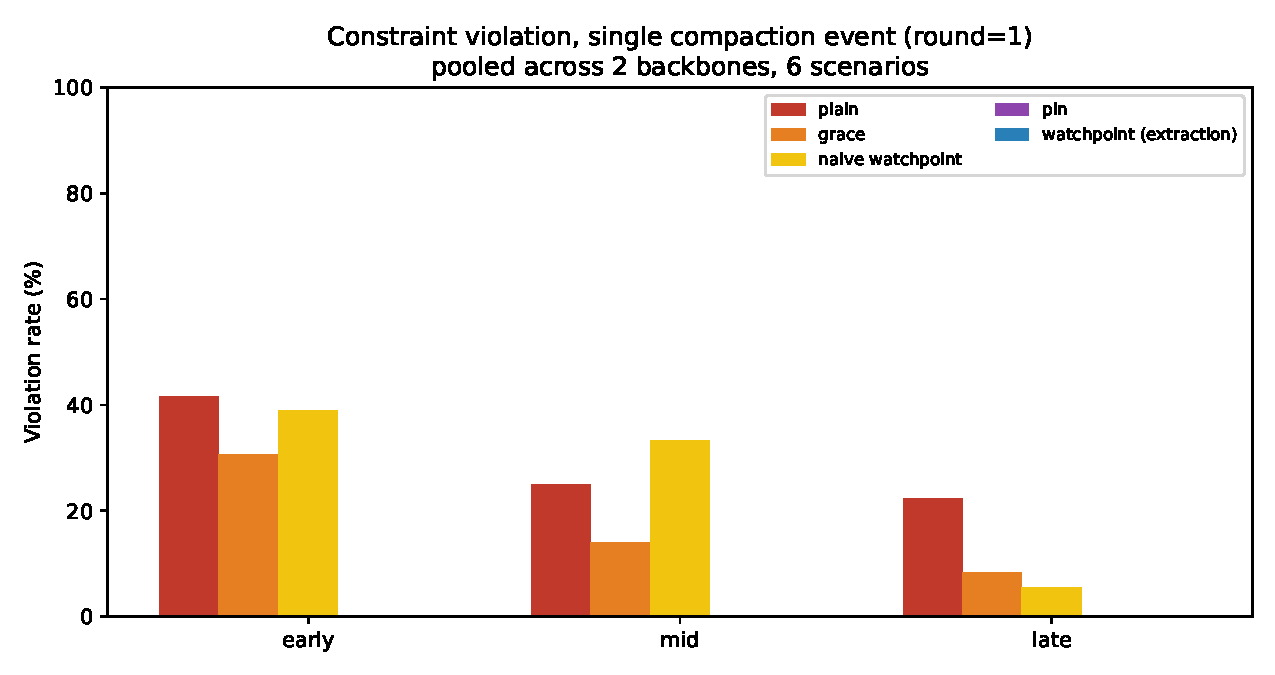
\includegraphics[width=0.85\textwidth]{fig4_exp1_round1_allmethods.pdf}
\caption{Constraint violation, single compaction event, by position and method.}
\label{fig:exp1round1}
\end{figure}

Under three rounds of recursive compaction (Table~\ref{tab:exp1round3}, Figure~\ref{fig:exp1round3}), plain violation rises sharply (as already established for this transcript design), the naive watchpoint recovers only part of that loss, and the extraction-based watchpoint again ties pin (both effectively 0 to 6\%, $p=0.49$ to $1$ at every position) while beating plain and the naive version by very large margins (plain comparisons $p<10^{-4}$ everywhere; naive comparisons $p<0.002$ everywhere).

\begin{table}[h]
\centering
\small
\begin{tabular}{lrrrr}
\toprule
Position & Plain & Naive watchpoint & Pin & Watchpoint \\
\midrule
Early & 83.3\% & 50.0\% & 0.0\% & \textbf{5.6\%} \\
Mid   & 80.6\% & 41.7\% & 0.0\% & \textbf{2.8\%} \\
Late  & 41.7\% & 33.3\% & 0.0\% & \textbf{2.8\%} \\
\bottomrule
\end{tabular}
\caption{Constraint violation rate under 3 recursive compaction rounds, pooled over 6 scenarios and 2 backbones (n=36 per cell).}
\label{tab:exp1round3}
\end{table}

\begin{figure}[h]
\centering
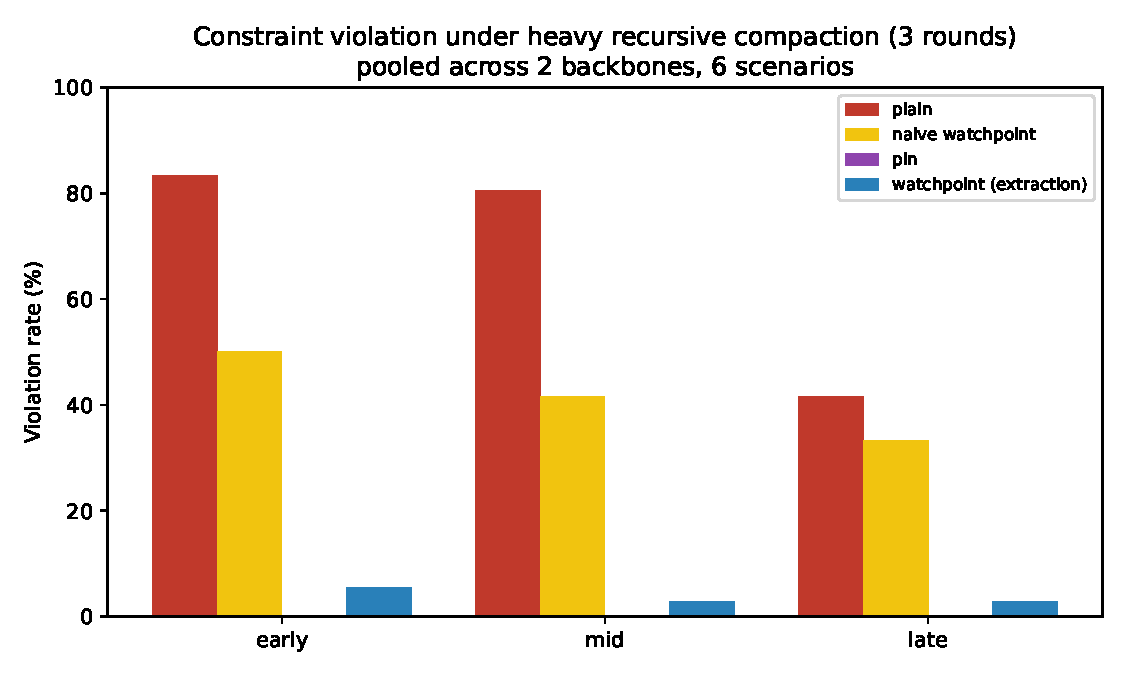
\includegraphics[width=0.75\textwidth]{fig5_exp1_round3_allmethods.pdf}
\caption{Constraint violation under 3 recursive compaction rounds, by position and method.}
\label{fig:exp1round3}
\end{figure}

The extraction-based watchpoint's patch rate is 97 to 100\% at both round counts (round 1: 36/36, 36/36, 35/36; round 3: 34/36, 35/36, 35/36, across early/mid/late), essentially indistinguishable from pin's unconditional 100\%. The naive version's patch rate, by contrast, is 0 to 8\% at round 1 and 8 to 42\% at round 3, which is exactly why it recovers so little of the loss it is supposed to catch.

\section{Experiment 2: Goal Resurrection}
\label{sec:exp2}

\subsection{Design}
Five goal-redirect scenarios that passed the floor and ceiling checks are each run at three redirect positions and four methods (plain, $k{=}2$; anchor; naive watchpoint; extraction watchpoint), one backbone, four repeats per cell.

\subsection{Results}

\begin{table}[h]
\centering
\small
\begin{tabular}{lrrrr}
\toprule
Position & Plain & Naive watchpoint & Anchor & Watchpoint \\
\midrule
Early & 70.0\% & 65.0\% & 95.0\% & \textbf{90.0\%} \\
Mid   & 85.0\% & 90.0\% & 95.0\% & \textbf{95.0\%} \\
Late  & 100.0\% & 85.0\% & 100.0\% & \textbf{100.0\%} \\
\bottomrule
\end{tabular}
\caption{Rate of correctly following the revised goal, by redirect position and method, pooled over 5 scenarios (n=20 per cell).}
\label{tab:exp2}
\end{table}

The extraction-based watchpoint statistically ties the anchor instruction at every position ($p=1$), something the grace buffer (Section~\ref{sec:exp1}, Figure~\ref{fig:exp1round1}'s analogue for this task) could not do. It is directionally better than plain at early and mid, though not significantly so at this sample size ($p\approx0.24$, $p=0.61$), and directionally, though again not significantly, better than the naive self-judgment version at every position ($p\approx0.13$, $p=1$, $p\approx0.23$). Figure~\ref{fig:exp2} shows all four methods together.

\begin{figure}[h]
\centering
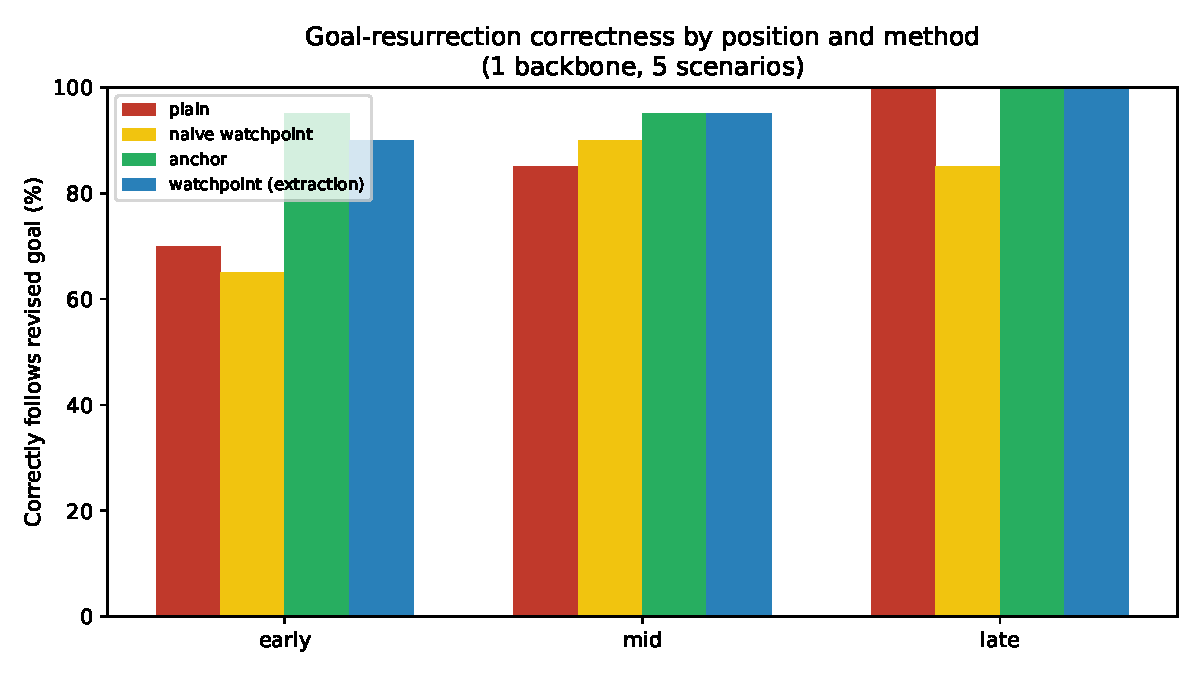
\includegraphics[width=0.85\textwidth]{fig6_exp2_allmethods.pdf}
\caption{Rate of correctly following the revised goal, by redirect position and method.}
\label{fig:exp2}
\end{figure}

The extraction-based watchpoint's patch rate here is 75\%, 50\%, and 85\% at early, mid, and late, markedly lower than the 97 to 100\% seen on the constraint task, meaning the check is genuinely selective on this task rather than saturating.

\section{Discussion}
\label{sec:discussion}

Two things distinguish Watchpoint Compaction from the two ad hoc fixes it replaces. First, generality: one mechanism, unchanged in its logic, ties the best existing fix on two structurally different failures, where each existing fix only worked on one. Second, and this is the part worth being precise about rather than glossing over, the mechanism's central selling point, that it should only pay a repair cost when something actually drifted, holds on one task and not the other.

On the constraint task, the well-calibrated check patches 97 to 100\% of the time. Once a check is strict enough to actually catch real drift, it turns out that ordinary single-pass summarization almost never preserves an arbitrary rule well enough to pass that check, so a properly calibrated watchpoint ends up behaving almost exactly like unconditional pinning, at the added cost of the audit call itself. For this failure type, Watchpoint Compaction is not a cheaper alternative to Constraint Pinning; it is a more complicated way of arriving at approximately the same policy, and a team building a real system should probably just pin.

On the goal task, the same check patches only 50 to 85\% of the time, meaningfully below saturation, and still matches the specialized anchor fix. The difference between the two tasks is structural. Constraint retention is a presence check: either the rule survived in some recognizable form or it did not, and a strict, well-calibrated check will say ``patch it'' almost every time because plain summarization rarely preserves an arbitrary rule perfectly. Goal resurrection is a disambiguation problem: the summary usually says \emph{something} about the objective, often the correct one, and the check only needs to intervene when the summary's implicit answer to ``which of two candidates'' is wrong, which happens less often than ``did an arbitrary fact survive verbatim.'' Self-verification earns its keep specifically on the second kind of problem. This suggests the mechanism's real target use case is not indiscriminately watching every rule a session has ever stated, which is what pinning already does perfectly well and more cheaply, but watching values that can drift between multiple valid-looking states, such as which of several possible goals, branches, or in-flight plans is the current one.

\section{Limitations}
\label{sec:limitations}

\textbf{Backbones.} Both models are inexpensive, open-weight backbones, not the frontier, closed-weight models that motivate the broader compaction research program this work sits inside. The goal-resurrection experiment additionally uses only one backbone; the constraint experiment's own finding that floor behavior is backbone-dependent (Section~\ref{sec:method}) suggests this should be checked on a second backbone before generalizing.

\textbf{Synthetic transcripts.} The filler pool does not involve real code, test failures, or tool execution, and a real coding agent's context has much higher-entropy content that a summarizer, and an extraction-based check, may treat differently.

\textbf{Grading is a structured-decision proxy}, not execution in a real environment, unlike ConstraintRot's deterministic tool-call grading \cite{governancedecay}.

\textbf{Keyword-based extraction matching is scenario-specific hand engineering}, even though it is far cheaper and more general than a goal-specific prompt: each scenario needed a chosen keyword or keyword set, checked in advance for discriminating correctly, and a fielded system would need a more automatic way to derive this, for instance an embedding-similarity or entailment check in place of exact keyword matching, which we did not have the budget to compare against keyword matching in this study.

\textbf{Small per-cell samples} (n=20 to 36) are enough to detect the large effects reported here but not smaller ones, and several directionally consistent comparisons in Experiment 2 do not reach significance at this sample size.

\textbf{The efficiency argument in Section~\ref{sec:discussion} is diagnosed, not solved.} We did not test whether a cheaper, more selective check (for instance, checking only rules with some prior evidence of ambiguity) could recover some of pinning's cost advantage on the constraint task without sacrificing watchpoint's cross-task generality; that is the natural next experiment.

\section{Conclusion}
\label{sec:conclusion}

Two known compaction failures, a dropped rule and a resurrected stale goal, each already had a working fix, and neither fix worked for the other's failure. We built one mechanism, Watchpoint Compaction, that works for both, and in doing so learned something more specific than ``self-verification helps'': a naive self-judgment check is actively misleading, missing nearly all the drift it exists to catch, in a way that lines up with an established result about model overconfidence rather than being a quirk of our setup; a properly built extraction-based check fixes this completely and statistically ties the best specialized fix on both failures; and that check's promised efficiency, paying only when something actually broke, materializes on the failure that requires disambiguating between competing candidates and not on the failure that only requires detecting whether one fact survived. The practical recommendation this leaves a harness builder with is correspondingly specific: pin rules, because a smarter mechanism buys nothing there once it is calibrated well enough to work at all, and watch goals, or anything else with more than one valid-looking current state, because that is where the selectivity, and the savings, are real.

\section*{Reproducibility}
Code and raw per-trial records for this study are available in the accompanying repository, alongside a broader research plan this paper is one part of.

\begin{thebibliography}{99}

\bibitem{anthropiccontext} Anthropic. Effective context engineering for AI agents. Anthropic Engineering blog, September 29, 2025. \url{https://www.anthropic.com/engineering/effective-context-engineering-for-ai-agents}

\bibitem{trace} TRACE: Trajectory-Relative Agent ContExt compression. arXiv:2608.06503, August 2026.

\bibitem{governancedecay} Governance Decay: How Context Compaction Silently Erases Safety Constraints in Long-Horizon LLM Agents (benchmark: ConstraintRot). arXiv:2606.22528, June 2026.

\bibitem{lostincompaction} Lost in Compaction. arXiv:2608.11242, July 2026.

\bibitem{compactioncliff} Compaction Cliff. arXiv:2608.22752, August 2026.

\bibitem{cliffcompaction} CliffCompaction: Cost-Efficient Compaction for Long-Horizon Coding Agents. arXiv:2609.26779, September 2026.

\bibitem{supersede} Supersede. arXiv:2606.27472, June 2026.

\bibitem{depguided} From Faulty Memories to Corrected Actions: Dependency-Guided Rollback Repair for Memory-Augmented Agents. arXiv:2608.10502, August 2026.

\end{thebibliography}

\end{document}
